\textbf{(Challenge Question)} A gambler has the opportunity to make bets on
the outcomes of a sequence of coin flips. If the coin comes up heads, she wins as many
dollars as she has staked on that flip; if it is tails, she loses her stake. The game ends
when the gambler wins by reaching her goal of \$100, or loses by running out of money.
On each flip, the gambler must decide what portion of her capital to stake, in integer
numbers of dollars. This problem can be formulated as an undiscounted, episodic, finite
MDP. The state is the gambler's capital, $s \in \{1, 2,..., 99\}$ and the actions
are stakes, $a \in \{0, 1,..., \min(s, 100-s) \}$.
The reward is +1 when reaching the goal of \$100 and zero on all other transitions. The probability of seeing heads is $p_h = 0.4$. 
%
\begin{enumerate}
  \item What does the value of a state mean in this problem? For example, in a gridworld where the value of 1 per step, the value represents the expected number of steps to goal. What does the value of state mean in the gambler's problem? Think about the minimum and maximum possible values, and think about the values of state 50 (which is $0.4$) and state 99 (which is near 0.95).
  \item Modify the pseudocode for value iteration to more efficiently solve this specific problem, by exploiting your knowledge of the dynamics. \textit{Hint: Not all states transition to every other state. For example, can you transition from state $1$ to state $99$?}  

\end{enumerate}
\begin{figure}[h!]
\centering
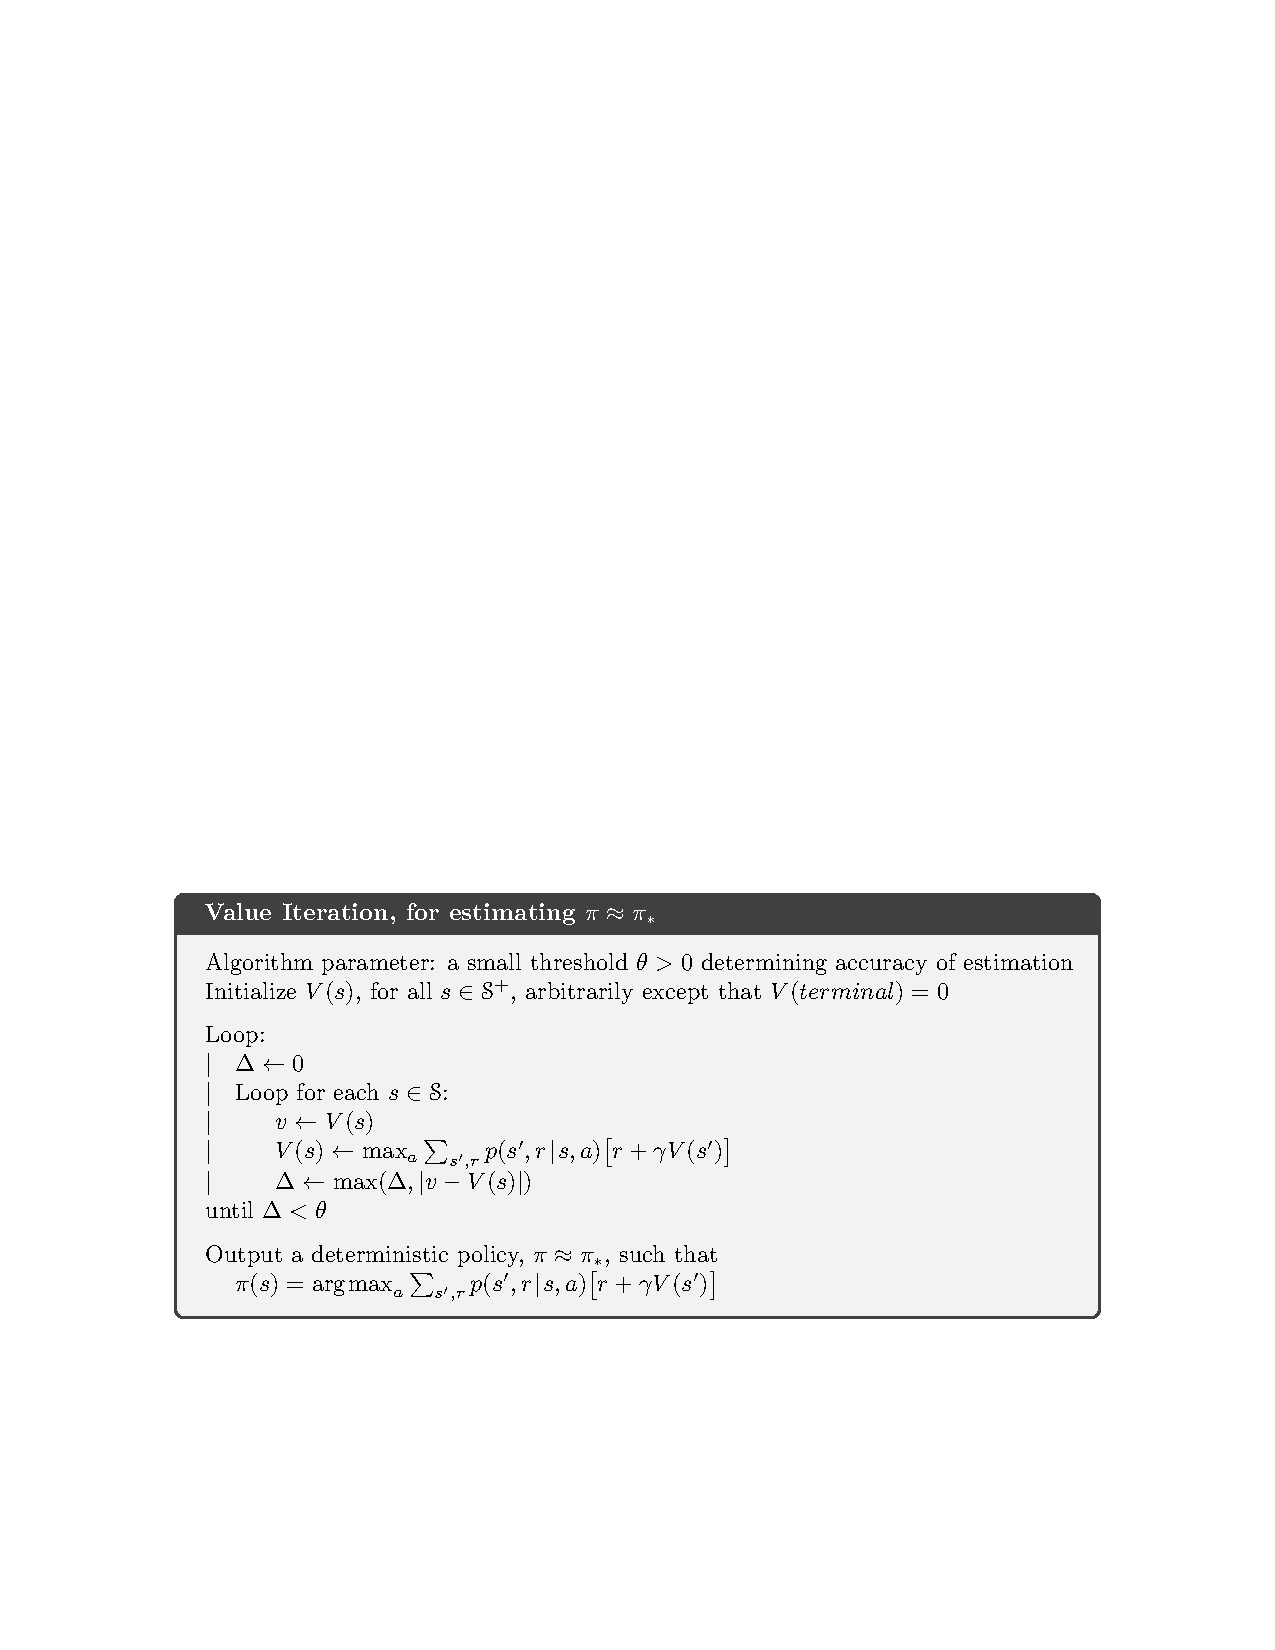
\includegraphics[scale=0.9]{figures/pseudocode_vi.pdf}
\end{figure}

%\bigspace